\documentclass[slidestop,compress,mathserif]{beamer}
%\documentclass[slidestop,compress,mathserif,handout]{beamer}

%\documentclass[xcolor=dvipsnames,handout]{beamer}
%\documentclass[xcolor=dvipsnames]{beamer}

%\documentclass[handout]{beamer}

%%% To get rid of solutions on handouts:
\newcommand{\soln}[1]{\textit{\textcolor{darkGray}{#1}}}				% For slides
%\newcommand{\soln}[1]{ }	% For handouts

% to get pausing to work properly on slides
\newcommand{\hide}[1]{#1}	% For slides
%\newcommand{\hide}[1]{ }	% For handouts


%\usepackage{multicol}
\usepackage{amsfonts}
%\usepackage[pdftex,dvipsnames]{color}
\usepackage{graphicx}
\usepackage{subfigure}
%\usepackage{picinpar}
\usepackage{pifont}
\usepackage{pgf,pgfarrows,pgfnodes}
%\usepackage{wasysym,manfnt,phaistos,empheq}
\usepackage[english]{babel}
\usepackage{pgfpages}
\usepackage{natbib}
\usepackage{hyperref}
\usepackage{multimedia}
%\usepackage{amsfonts,amstext,amssymb,amsbsy,amsopn,amsthm,eucal,latexsym,mathrsfs}
\usepackage{amsmath,amsfonts,amstext,amssymb,amsbsy,amsopn,amsthm,eucal,latexsym,mathrsfs}
\usepackage{ulem}
\usepackage{setspace}
\usepackage{array}
%\usepackage{rotating}
\usepackage{multirow}
\usepackage{verbatim}
\usepackage{multicol}

\setbeamertemplate{navigation symbols}{}

%\usepackage{tikz}
%\usetikzlibrary{arrows,shapes,trees,backgrounds}


%\setbeameroption{show notes on second screen}
%\setbeameroption{show notes}
%\setbeameroption{show only notes}

\definecolor{links}{HTML}{2A1B81}
\hypersetup{colorlinks,linkcolor=,urlcolor=links}

\newtheorem*{principle}{Inscrutibility Principle}
\newtheorem*{punchline}{Punch Line}
\newtheorem{defn}{Definition}

\definecolor{Scarlet}{RGB}{140,17,17}
\definecolor{VassarRed}{RGB}{128,0,0}

% "dinglist" environment
  \renewenvironment{dinglist}[2][blue]
  {\begin{list}{\textcolor{blue}{\ding{#2}}}{}}{\end{list}}
  % Symbol definitions for these lists
  \newcommand{\DingListSymbolA}{43}
  \newcommand{\DingListSymbolB}{243}
  \newcommand{\DingListSymbolC}{224}
  \newcommand{\DingListSymbolD}{219}
  \newcommand{\DingListSymbolCheck}{52}
  \newcommand{\DingListSymbolCross}{56}


  \newenvironment{ballotenv}
{\only{%
\setbeamertemplate{itemize item}{\ding{45}}%
\setbeamertemplate{itemize subitem}{\ding{46}}%
\setbeamertemplate{itemize subsubitem}{\ding{46}}}} {}
\setbeamertemplate{itemize item}{\ding{49}}
\setbeamertemplate{itemize subitem}{\ding{47}}
\setbeamertemplate{itemize subsubitem}{\ding{47}}


%User defined colors: See colors section
\xdefinecolor{oiBlue}{rgb}{0.15, 0.35, 0.55}
\xdefinecolor{gray}{rgb}{0.5, 0.5, 0.5}
\xdefinecolor{darkGray}{rgb}{0.3, 0.3, 0.3}
\xdefinecolor{darkerGray}{rgb}{0.2, 0.2, 0.2}
\xdefinecolor{rubineRed}{rgb}{0.89,0,0.30}
\xdefinecolor{linkCol}{rgb}{0.11,0.49,0.95}	
\xdefinecolor{irishGreen}{rgb}{0,0.60,0}	
\xdefinecolor{darkturquoise}{rgb}{0.44, 0.58, 0.86}
\definecolor{lightGreen}{rgb}{0.533,0.765,0.42}
\xdefinecolor{Regalia}{HTML}{522D80}
\xdefinecolor{ClemsonOrange}{HTML}{EA6A20}

\definecolor{duke@LightGrey}{RGB}{200,200,200}\definecolor{DarkGreen}{RGB}{0,100,0}
\definecolor{Oranges}{RGB}{255,127,0}
\definecolor{LightGray}{RGB}{211,211,211}

%\setbeamertemplate{footline}{%
%  \raisebox{5pt}{\makebox[\paperwidth]{\hfill\makebox[10pt]{\scriptsize\insertframenumber}}}}

\setbeamercolor{equation background}{fg=black,bg=duke@LightGrey}
  % Boxed equation
  \newcommand{\eqbox}[2][0.6]{%
  \centerline{
  \begin{beamerboxesrounded}[lower=equation background,width=#1\hsize,shadow=true]{}
\parbox{#1\hsize}{%
      \[
        \textcolor{black} {#2}
      \]}
  \end{beamerboxesrounded}
}}

\AtBeginSection[] {
  \begin{frame}<beamer>\frametitle{Outline}
    \tableofcontents[currentsection,hideothersubsections]
  \end{frame}
}
%
%
%\AtBeginSubsection[] {
%  \begin{frame}<beamer>\frametitle{Outline}
%    \tableofcontents%[currentsection,currentsubsection]
%  \end{frame}
%}

%\usecolortheme[RGB={82,45,128}]{structure}
%\usecolortheme[RGB={162,80,22}]{structure}
\usecolortheme[RGB={128,0,0}]{structure}
\usetheme[secheader]{Boadilla}
%\usetheme[height=7mm]{Rochester}
%\usetheme{Copenhagen}
%\usetheme{Antibes}
%\usecolortheme{seahorse}
%\usecolortheme{crane}
%\usecolortheme{rose}
%\usefonttheme[onlylarge]{structurebold}
%\usefonttheme[onlymath]{serif}



\def\diag{{\rm diag}}


\def\E{\mathbb{E}}
\def\Prob{\mathbb{P}}
\def\argmin{{\rm argmin}}
\def\argmax{{\rm argmax}}
\def\Def{\stackrel{def}{=}}


\newtheorem{assumption}{Assumptions}
\newtheorem*{proposition}{Proposition}
\newtheorem*{remark}{Remark}



%\setbeamercolor{disc title}{bg=oiBlue!40!white!60,fg=blue}
\setbeamercolor{disc body}{bg= Regalia!20!white!80,fg= Regalia!80!black!90}

\setbeamercolor{clicker ungraded title}{bg=irishGreen!80!white!50,fg=irishGreen!30!black!90}
\setbeamercolor{clicker ungraded body}{bg=irishGreen!20!white!80,fg=irishGreen!30!black!90}

\setbeamercolor{clicker review title}{bg=gray!80!white!80,fg=oiBlue!80!black!90}
\setbeamercolor{clicker review body}{bg=gray!30!white!90,fg=oiBlue!80!black!90}

\setbeamercolor{code body}{bg=gray!20!white!80,fg=black}


% Custom commands
\newcommand{\degree}{\ensuremath{^\circ}}
\newcommand{\Note}[1]{
\rule{2.5cm}{0.25pt} \\ \textit{\scriptsize {\textcolor{rubineRed}{Note:} \textcolor{gray}{#1}}}}
\newcommand{\ct}[1]{
\vfill
{\tiny #1}}
\newcommand{\Remember}[1]{\textit{\scriptsize{\textcolor{orange}{Remember:} \textcolor{gray}{#1}}}}
\newcommand{\red}[1]{\textit{\textcolor{rubineRed}{#1}}}
\newcommand{\pink}[1]{\textit{\textcolor{rubineRed!90!white!50}{#1}}}
\newcommand{\green}[1]{\textit{\textcolor{irishGreen}{#1}}}
\newcommand{\webURL}[1]{\urlstyle{same}\textit{\textcolor{linkCol}{\url{#1}}} }
\newcommand{\webLink}[2]{\href{#1}{\textcolor{linkCol}{{#2}}}}
\newcommand{\mail}[1]{\href{mailto:#1}{\textit{\textcolor{linkCol}{#1}}}}
\newcommand{\hl}[1]{\textit{\textcolor{oiBlue}{#1}}}
\newcommand{\hlGr}[1]{\textit{\textcolor{lightGreen}{#1}}}
\newcommand{\mathhl}[1]{\textcolor{oiBlue}{\ensuremath{#1}}}
\newcommand{\ex}[1]{\textcolor{blue}{{{\small (#1)}}}}
\newcommand{\disc}[1]{
\begin{beamerboxesrounded}[shadow = true, lower = disc body, upper = disc title]{}
#1
\end{beamerboxesrounded}
}

\newcommand{\cl}[1]{
\begin{beamerboxesrounded}[shadow = true, lower = clicker ungraded body, upper = clicker ungraded title]{Question}
$\:$ \\
#1
\end{beamerboxesrounded}
}

\newcommand{\clR}[1]{
\begin{beamerboxesrounded}[shadow = true, lower = clicker review body, upper = clicker review title]{\red{Review question} }
$\:$ \\
#1
\end{beamerboxesrounded}
}

\newcommand{\formula}[2]{
\begin{beamerboxesrounded}[shadow = true, lower = white, upper = clicker review body]{#1}
#2
\end{beamerboxesrounded}
$\:$ \\
}

\newenvironment{twocol}[4]{
\begin{columns}[c]
\column{#1\textwidth}
#3
\column{#2\textwidth}
#4
\end{columns}
}


\newenvironment{slot}[2]{
\begin{array}{c}
\underline{#1} \\
#2
\end{array}
}

\newcommand{\pr}[1]{
\left( #1 \right)
}

\newcommand{\solnMult}[1]{
\item[] \vspace{-0.59cm}
\only<beamer| beamer:1>{\item #1}
\soln{\only<2->{\item \red{#1}}}
}

%\newcommand{\codechunk}[1]{
%\begin{beamerboxesrounded}[shadow = true, lower = code body]{}
%{\small #1}
%\end{beamerboxesrounded}
%}

% Change margin

\newenvironment{changemargin}[2]{%
\begin{list}{}{%
\setlength{\topsep}{0pt}%
\setlength{\leftmargin}{#1}%
\setlength{\rightmargin}{#2}%
\setlength{\listparindent}{\parindent}%
\setlength{\itemindent}{\parindent}%
\setlength{\parsep}{\parskip}%
}%
\item[]}{\end{list}}

% Footnote

\long\def\symbolfootnote[#1]#2{\begingroup%
\def\thefootnote{\fnsymbol{footnote}}\footnote[#1]{#2}\endgroup}

% Commands from the book
\newenvironment{data}[1]{\texttt{#1}}{}
\newenvironment{var}[1]{\texttt{#1}}{}
\newenvironment{resp}[1]{\texttt{#1}}{}






%%%%%%%%%%%%%%%%%%%%%%%%%%%%%%%%%%%%%%%%%%%%%%%%%%%%%%%%%%%%%%%%%%%%%%%%%%%%%%%%%%%%%%%%%%%%%%%
\title[Chapter 5 part 2]{Chapter 5 part 2}
\subtitle{Continuous Random Variables}

%%%%%%%%%%%%%%%%%%%%%%%%%%%%%%%%%%%%%%%%%%%%%%%%%%%%%%%%%%%%%%%%%%%%%%%%%%%%%%%%%%%%%%%%%%%%%%%


\author[Jingchen (Monika) Hu] % (optional, use only with lots of authors)
{Jingchen (Monika) Hu}
% - Give the names in the same order as the appear in the paper.
% - Use the \inst{?} command only if the authors have different
%   affiliation.

\institute[Vassar] % (optional, but mostly needed)
{Vassar College}
% - Use the \inst command only if there are several affiliations.
% - Keep it simple, no one is interested in your street address.

\date[MATH 241] % (optional, should be abbreviation of conference name)
{MATH 241}
% - Either use conference name or its abbreviation.
% - Not really informative to the audience, more for people (including
%   yourself) who are reading the slides online

\subject{MATH 241}
% This is only inserted into the PDF information catalog. Can be left
% out.



% If you wish to uncover everything in a step-wise fashion, uncomment
% the following command:

%\beamerdefaultoverlayspecification{<+->}



\begin{document}




%%%%%%%%%%%%%%%%%%%%%

% Title Page

\begin{frame}%[plain]
\titlepage
\end{frame}


%%%%%%%%%%%%%%%%%%%%%%%%%%%%%%%%%%%%%%%%%%
%\addtocounter{framenumber}{-1}
%\begin{frame}{Midterm Feedback}
%\begin{columns}[T]
%\begin{column}{4cm}
%\vspace{-1cm}
%\begin{figure}
%\centering
%\includegraphics[width=5cm,height=8cm]{figures/feedback_barplots}
%\end{figure}
%\end{column}
%\begin{column}{7.8cm}
%\vspace{-0.3cm}
%{\pause
%\small \centerline{\underline{\textbf{Likes}}}}
%{%\footnotesize
%\begin{itemize}
%\item Lecture: well-organized, informative, \\
%clear expectation, good balance between theory and practice
%%in-class questions are  %\\``one of the best math classes"
%\item Slides: well-prepared, easy to follow
%%\item In-class questions: very helpful
%\item Homework \& quizzes: good practice
%\item In-class questions: helpful %in understanding concepts
%\item Exam \& quizzes: fair in difficulty
%\item ``Somewhat challenging but not too much''
%%\item Willingness to help%Available outside of classroom %office hour
%%\item Lab: interesting, practical programming skill, solidify core concepts
%\end{itemize}
%}
%{\pause
%\small \centerline{\underline{\textbf{To improve}}}}
%{%\footnotesize
%\begin{itemize}
%%\item Detailed expectation on the programming software (R) in syllabus
%\item Examples in class: more similar to HW %(harder)
%\item Homework solutions
%\item Practice exam
%%\item Post slides 12 hours before class
%%\item Go over commonly missed homework in class
%%\item Increase participation for in-class questions
%%\item More in-class activities (?)
%%\item More explanation in labs
%%\item More video?
%%\item Slides on Sakai: same slides or handout?
%%\item More practice, more examples
%%\item Some other detailed suggestions...
%
%\end{itemize}
%}
%\end{column}
%\end{columns}
%\end{frame}


%%%%%%%%%%%%%%%%%%%%%%
%\addtocounter{framenumber}{-1}
%
%\begin{frame}\frametitle{Annoucement}
%
%\begin{itemize}
%%\item HW5: \red{due now!}
%\item HW6: \red{due Thursday, Oct 23nd}
%
%\vspace{0.5cm}
%
%
%
%\end{itemize}
%%\begin{center}
%%\includegraphics[width = \textwidth]{figures/midterm_score}
%%\end{center}
%
%
%\end{frame}



%%%%%%%%%%%%%%%%%%%%%%
\begin{frame}{Outline}
%\tableofcontents[hideallsubsections,pausections]
\tableofcontents[hideallsubsections]
\end{frame}

%%%%%%%%%%%%%%%%%%%%%%%%%%%%%%%%%%%%%%%%%%
\section{Normal distribution}
%%%%%%%%%%%%%%%%%%%%%%%%%%%%%%%%%%%%%%%%%%

\begin{frame}
\frametitle{Normal Distribution}

\vspace{-0.2cm}
\begin{defn}
A continuous random variable $X$ has a \hl{Normal distribution} distribution with mean $\mu$ and variance $\sigma^2$ if its pdf is
%\vspace{-0.3cm}
\[
X \sim \text{N}(\mu, \sigma^2) \Longleftrightarrow
 f(x) = \frac{1}{\sqrt{2\pi\sigma^2}}~e^{ -\frac{(x-\mu)^2}{2\sigma^2} }, \text{ where } x \in \mathbb{R}
\]
\end{defn}

\pause
Pdf: unimodal and symmetric, bell shaped continuous random variable
\begin{center}
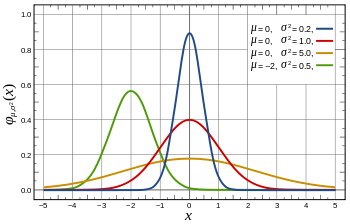
\includegraphics[width = 0.5\textwidth]{figures/normal_pdf}
\end{center}

\end{frame}


%%%%%%%%%%%%%%%%%%%%%%%%%%%%%%%%%%%%%
%\addtocounter{framenumber}{-1}
%\begin{frame}
%\frametitle{Get yourself a 10 Deutsche Mark bill}
%
%\begin{center}
%
\includegraphics[width=\textwidth]{figures/deutsche_mark}
%\end{center}
%
%\end{frame}


%%%%%%%%%%%%%%%%%%%%%%%%%%%%%%%%%%%%%%%%%%
\begin{frame}\frametitle{The normal pdf is well-defined} %$f(x)= \frac{1}{\sqrt{2\pi\sigma^2}}~e^{ -\frac{1}{2}\frac{(x-\mu)^2}{\sigma^2} }$}
({\color{red}not required})
\[\int_{-\infty}^\infty \frac{1}{\sqrt{2\pi\sigma^2}}~e^{ -\frac{(x-\mu)^2}{2\sigma^2} } dx =1 \]
\disc{Use the fact that normal pdf is well define, calculate the integral
\[
\int_{-\infty}^{\infty} e^{-\frac{(x -1)^2}{10}}dx = ?
\]
}
\pause
Suppose we have a random variable $X \sim \text{N}(\mu = 1, \sigma^2 = 5)$, then
\[
1  = \int_{-\infty}^\infty \frac{1}{\sqrt{2\pi\sigma^2}}~e^{ -\frac{(x-\mu)^2}{2\sigma^2} } dx
 = \int_{-\infty}^{\infty} \frac{1}{\sqrt{2 \pi \cdot 5}}~e^{-\frac{(x -1)^2}{10}}dx\]
 \pause
 \[\Longrightarrow \int_{-\infty}^{\infty} e^{-\frac{(x -1)^2}{10}}dx = \sqrt{10\pi}\]


%\red{Proof}
%
%%\invisible{
%\pause%\footnotesize{
%It's suffice to show that the pdf of the standard normal $\phi(x)$ is well-defined, i.e.
%\[ \int_{-\infty}^\infty \frac{1}{\sqrt{2\pi}}~ e^{-\frac{x^2}{2}}dx = 1 \Longleftrightarrow
%I = \int_{-\infty}^\infty  e^{-\frac{x^2}{2}}dx = \sqrt{2\pi}\]
%\pause
%\begin{align*}
%\uncover<3->{
%I^2  & = \int_{-\infty}^\infty  e^{-\frac{x^2}{2}}dx \cdot \int_{-\infty}^\infty  e^{-\frac{y^2}{2}}dy
% = \int_{-\infty}^\infty \int_{-\infty}^\infty e^{-\frac{x^2 + y^2}{2}}dx dy\\
% }
%\uncover<4->{
%(\text{Polar swap: } &   x = r\cos\theta, y = r\sin\theta, \text{ then } x^2 + y^2 = r^2, dxdy = r d\theta dr)  \\
%}
%\uncover<5->{
%& = \int_{0}^\infty \int_{0}^{2\pi} re^{-\frac{r^2}{2}}d\theta dr =  2\pi \int_{0}^\infty  re^{-\frac{r^2}{2}} dr\\
%& = 2\pi \int_{0}^\infty  e^{-\frac{r^2}{2}} d\left(\frac{r^2}{2}\right) = - 2\pi  \left. e^{-\frac{r^2}{2}} \right|_{0}^\infty = 2\pi
%}
%\end{align*}

%}
%}




\end{frame}




%%%%%%%%%%%%%%%%%%%%%%%%%%%%%%%%%%%%

\begin{frame}
\frametitle{Normal distributions with different parameters}

\vspace{-1cm}
\begin{center}
\[N(\mu = 0, \sigma^2 = 1) \hspace{1.4cm} N(\mu = 19, \sigma^2 = 16) \]
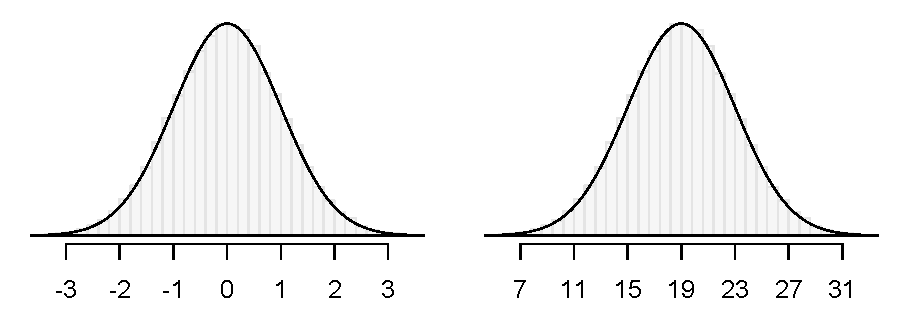
\includegraphics[width=0.7\textwidth]{figures/twoSampleNormals}
\end{center}

\begin{center}
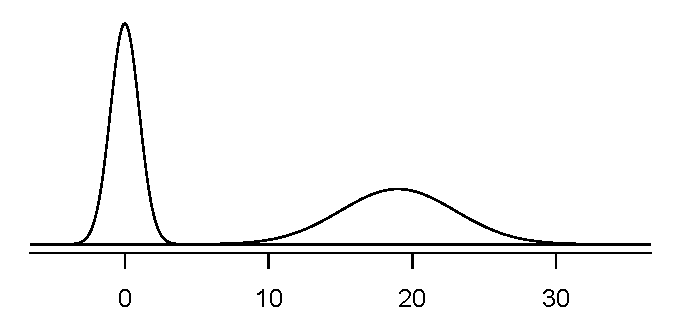
\includegraphics[width=0.7\textwidth]{figures/twoSampleNormalsStacked}
\end{center}

\end{frame}

%%%%%%%%%%%%%%%%%%%%%%%%%%%%%%%%%%%%%%%%%%
\begin{frame}\frametitle{Mean and variance of Normal random variable}
If $X \sim \text{N}(\mu, \sigma^2)$, and $Z = \frac{X - \mu}{\sigma}$, then $Z$ has a standard normal distribution (more later in Chapter 5.7).
%\vspace{-0.2cm}
\[ Z \sim \text{N}(0, 1) \]
%\red{Proof}
\pause

\begin{itemize}
\item $E[X] = \mu$ ({\color{red} required})
\end{itemize}
\pause


%\red{Proof}
%\invisible{
%\pause
\hspace{0.5cm}
Since $X \sim \text{N}(\mu, \sigma^2) \Longleftrightarrow X = \sigma Z + \mu$ and $Z \sim \text{N}(0, 1)$,
it's suffice to show the mean and variance of standard normal are $0$ and $1$.
\pause
{\footnotesize{
\begin{align*}
E[Z] & = \int_{-\infty}^{\infty} x f_Z(x) dx = \int_{-\infty}^{\infty} x \frac{1}{\sqrt{2\pi}} e^{-\frac{x^2}{2}}dx\\
& = \frac{1}{\sqrt{2\pi}}\int_{-\infty}^{\infty} x~e^{-\frac{x^2}{2}}dx\\
& = -\frac{1}{\sqrt{2\pi}}\left. e^{-\frac{x^2}{2}}\right|_{-\infty}^{\infty} = 0
\end{align*}
}}
%}

\end{frame}

%%%%%%%%%%%%%%%%%%%%%%%%%%%%%%%%%%%%%%%%%%
\begin{frame}\frametitle{Mean and variance of Normal random variable}
If $X \sim \text{N}(\mu, \sigma^2)$, and $Z = \frac{X - \mu}{\sigma}$, then $Z$ has a standard normal distribution (more later in Chapter 5.7).
%\vspace{-0.2cm}
\[ Z \sim \text{N}(0, 1) \]
%\red{Proof}

\begin{itemize}
\item $Var(X) = \sigma^2$ ({\color{red} required})
\end{itemize}


%\red{Proof}
%\invisible{
%\pause
\hspace{0.5cm}
Since $X \sim \text{N}(\mu, \sigma^2) \Longleftrightarrow X = \sigma Z + \mu$ and $Z \sim \text{N}(0, 1)$,
it's suffice to show the mean and variance of standard normal are $0$ and $1$.

\pause
{\footnotesize{
\begin{align*}
Var[Z] & = E[Z^2]  - (E[Z])^2 = E[Z^2] = \int_{-\infty}^{\infty} x^2 f_Z(x) dx = \int_{-\infty}^{\infty} x^2 \frac{1}{\sqrt{2\pi}} e^{-\frac{x^2}{2}}dx\\
& = \frac{1}{\sqrt{2\pi}}\int_{-\infty}^{\infty} x^2~e^{-\frac{x^2}{2}}dx \,\,\, (\text{integration by parts}: u = x, dv = xe^{-x^2/2}dx) \\
& = \frac{1}{\sqrt{2\pi}}\left\{  - \left. xe^{-\frac{x^2}{2}}\right|_{-\infty}^{\infty} + \int_{-\infty}^{\infty} e^{-\frac{x^2}{2}}dx\right\}\\
& = \int_{-\infty}^{\infty} \frac{1}{\sqrt{2\pi}}e^{-\frac{x^2}{2}}dx =1
\end{align*}
}}

\end{frame}


%%%%%%%%%%%%%%%%%%%%%%%%%%%%%%%%%%%%

\begin{frame}
\frametitle{68-95-99.7 Rule}

\begin{itemize}

\item A random variable $X$ has a normal distribution,
\begin{itemize}
\item about 68\% probability $X$ falls within 1 SD of the mean,
\item about 95\% probability $X$ falls within 2 SD of the mean,
\item about 99.7\% probability $X$ falls within 3 SD of the mean.
\end{itemize}

\item The probability of $X$ falls 4, 5, or more standard deviations away from the mean is very low.

\end{itemize}

\begin{center}
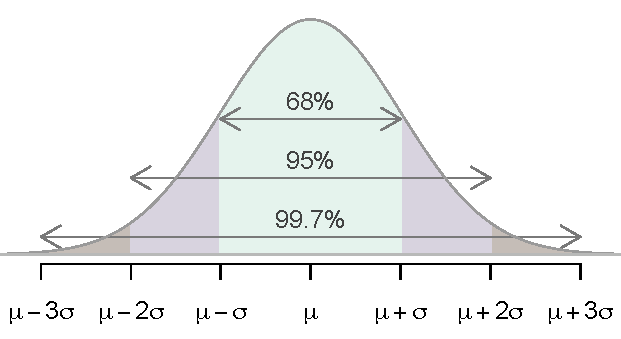
\includegraphics[width=0.7\textwidth]{figures/6895997}
\end{center}

\end{frame}




%%%%%%%%%%%%%%%%%%%%%%%%%%%%%%%%%%%%%%%%%%
\begin{frame}\frametitle{Normal probability calculation}
\begin{itemize}
%\item If $X \sim \text{N}(\mu, \sigma^2)$, and $Z = \frac{X - \mu}{\sigma}$, then $Z$ has a standard normal distribution.
%%\vspace{-0.2cm}
%\[ Z \sim \text{N}(0, 1) \]
%%\red{Proof}
%\pause
%We are going to show this later, when we learn Chapter 5.7.

%%\invisible{
%\pause\vspace{-0.5cm}%\footnotesize{
%\[ X  = \sigma Z + \mu  \Longrightarrow \]
%\[ F_Z(z)   = P(Z \leq z) = P(X \leq \sigma z + \mu) = F_X(\sigma z + \mu) \]
%\pause\vspace{-0.5cm}
%\begin{align*}
%f_Z(z) &  = \frac{d}{dz}F_Z(z) =  \frac{d}{dz} F_X(\sigma z + \mu)\\
%\text{\red{(chain rule)}}  &  =  f_X(\sigma z + \mu) \cdot \frac{d}{dz} (\sigma z + \mu)\\
%& =  \frac{1}{\sqrt{2\pi\sigma^2}}~e^{ -\frac{1}{2}\frac{(\sigma z + \mu-\mu)^2}{\sigma^2} } \cdot \sigma
% =  \frac{1}{\sqrt{2\pi}}~e^{ -\frac{1}{2}z^2 }
%\end{align*}
%%}
%%}

%\pause
\item We denote $\phi(x)$ and $\Phi(x)$ as pdf and cdf of the standard normal distribution respectively.
\pause
\item Probability calculations for $X$ in terms of $Z$:
\begin{align*}
P(a < X < b) %&= P\left(\frac{a - \mu}{\sigma} < \frac{X - \mu}{\sigma} \leq \frac{b - \mu}{\sigma}\right)\\
&= P\left(\frac{a - \mu}{\sigma} < Z < \frac{b - \mu}{\sigma}\right) \\
%&= P\left(Z \leq \frac{b - \mu}{\sigma} \right) - P\left(Z \leq \frac{a - \mu}{\sigma}\right) \\
& = \Phi\left(\frac{b - \mu}{\sigma}\right) - \Phi\left(\frac{a - \mu}{\sigma}\right)
\end{align*}


\end{itemize}
\end{frame}


%%%%%%%%%%%%%%%%%%%%%%%%%%%%%%%%%%%%
\begin{frame}

\disc{{At Heinz ketchup factory the amounts which go into bottles of ketchup are supposed to be normally distributed with mean 36 oz. and standard deviation 0.11 oz. Once every 30 minutes a bottle is selected from the production line, and its contents are noted precisely. If the amount of ketchup in the bottle is below 35.8 oz. or above 36.2 oz., then the bottle will fails the quality control inspection. What's the probability that the amount of ketchup in a randomly selected bottle is less than 35.8 ounces?}}

$\:$

\pause

Let $X$ = amount of ketchup in a bottle: $X \sim N(36, 0.11^2)$

\pause

\begin{center}
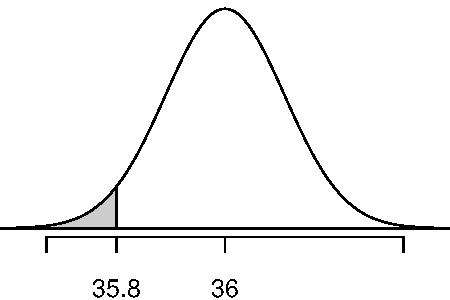
\includegraphics[width=0.45\textwidth]{figures/ketchupLT358}
\end{center}

\end{frame}

%%%%%%%%%%%%%%%%%%%%%%%%%%%%%%%%%%%%

\begin{frame}


\[z = \frac{x - \mu}{\sigma} = \frac{35.8 - 36}{0.11} = -1.82 \]

\[ P(X < 35.8) = P(Z < -1.82) = 0.0344 \]

\vspace{0.5cm}
\pause

\begin{center}
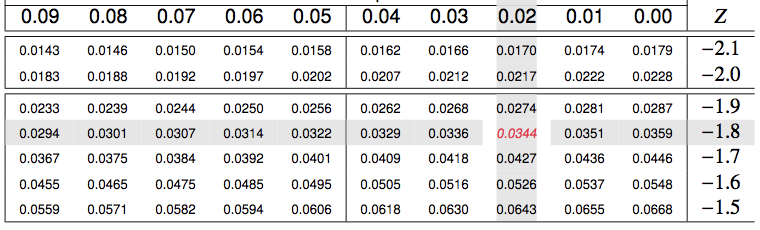
\includegraphics[width=\textwidth]{figures/NormalTable2}
\end{center}

\end{frame}



%%%%%%%%%%%%%%%%%%%%%%%%%%%%%%%%%%%%%%%%%%%
\begin{frame}
\frametitle{Normal approximation to the Binomial distribution}

\vspace{-0.5cm}
\begin{center}
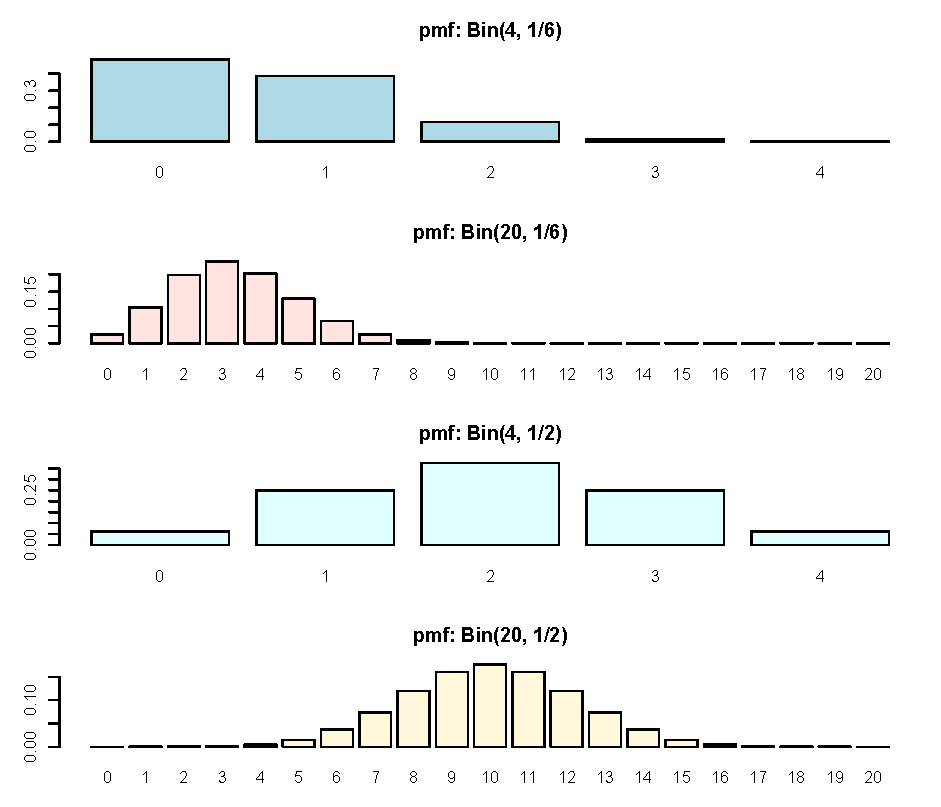
\includegraphics[scale = 0.6]{figures/pmf2}
\end{center}

\end{frame}
%%%%%%%%%%%%%%%%%%%%%%%%%%%%%%%%%%%%%%%%%%



\begin{frame}
\frametitle{Normal approximation to the Binomial distribution}

Let $X \sim \text{Bin}(n, p)$.
When $n$ is large enough, or more specifically, $np (1-p) \geq 10$,
the binomial distribution can be approximated by the normal distribution
\[ P(X = i) \approx P(i - 0.5 < Y < i + 0.5), \quad Y \sim \text{N}(\mu, \sigma^2) \]
with parameters $\mu = np$ and $\sigma^2 = np(1-p)$.

\pause
\begin{itemize}
\item Probability calculation (actually, approximation)
\begin{align*}
P(a \leq X \leq b) &\approx P(a - 0.5 < Y < b + 0.5) \\
& = P\left( \frac{a - 0.5 - np}{\sqrt{np(1-p)}} < \frac{Y - \mu}{\sigma} < \frac{b + 0.5 - np}{\sqrt{np(1-p)}} \right)\\
& = \Phi\left( \frac{b + 0.5 - np}{\sqrt{np(1-p)}} \right) -  \Phi\left( \frac{a - 0.5 - np}{\sqrt{np(1-p)}} \right)
\end{align*}



\end{itemize}

\end{frame}


%%%%%%%%%%%%%%%%%%%%%%%%%%%%%%%%%%%%

\begin{frame}
\frametitle{}

\disc{The ideal size of a first-year class at a particular college is 150 students. The college, knowing from past experience that, on the average, only 30 percent of those accepted for admission will actually attend, uses a policy of approving the applications of 450 students. Compute the probability that more than 150 first-year students attend this college.}
\pause

\begin{itemize}
\item We are given that $X \sim \text{Bin}(n =450, p = 0.3)$, and we are asked for the probability
\[
P(X > 150) = p(151) + \cdots + p(450) = 1 - p(0) - p(1) - \cdots - p(151)
\]

\item \pause To use normal approximation, first check conditions
\[ np(1-p) = 450 \times 0.3 \times 0.7 = 94.5 \geq 10\]
\end{itemize}

\end{frame}

%%%%%%%%%%%%%%%%%%%%%%%%%%%%%%%%%%%%

\begin{frame}

Use Normal approximation with continuity correction,

\begin{align*}
P(X > 150) & \approx P(X > 150 + 0.5)\\
& = P\left(Z > \frac{\red{150.5} - 450(0.3)}{\sqrt{450(0.3)(0.7)}}\right)\\
& = P(Z > 1.59) \\
&= 1 - 0.9441 = 0.0559
\end{align*}

\end{frame}



%%%%%%%%%%%%%%%%%%%%%%%%%%%%%%%%%%%%%%%%%%
\begin{frame}\frametitle{Recap: Normal distribution $X \sim \text{N}(\mu, \sigma^2)$}

\twocol{0.25}{0.75}
{
\begin{center}
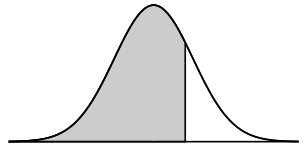
\includegraphics[scale = 0.3]{figures/cdf_pos}
\end{center}
\begin{center}
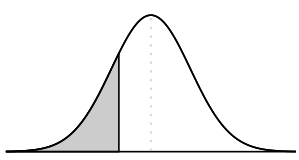
\includegraphics[scale = 0.3]{figures/cdf_neg}
\end{center}
}
{
 %(or Gaussian distribution)
\begin{itemize}
%\vspace{0.2cm}
%\item Pdf \vspace{-0.5cm}
%\[f(x) = \frac{1}{\sqrt{2\pi\sigma^2}}~e^{ -\frac{(x-\mu)^2}{2\sigma^2} } \]
\item Mean $\mu$, variance $\sigma^2$
\item Symmetry \vspace{-0.2cm}
\[ f(\mu-x) = f(\mu+x), F(\mu-x) = 1 - F(\mu+x) \]
\item \pause\vspace{-0.2cm}
Standard normal distribution $\mu = 0, \sigma^2 = 1$. \vspace{-0.2cm}
\[ X \sim \text{N}(\mu, \sigma^2) \Longleftrightarrow Z = \frac{X - \mu}{\sigma} \sim \text{N}(0, 1)\]
\item \vspace{-0.2cm}
Find probability using $\Phi(\cdot)$ table \vspace{-0.2cm}
\[ P(a< X < b) = \Phi\left( \frac{b - \mu}{\sigma}\right) - \Phi\left( \frac{a - \mu}{\sigma}\right) \]
\item \pause\vspace{-0.2cm}
Normal approximation to Binomial $X \sim \text{Bin}(n, p)$ \vspace{-0.2cm}
\[ Y \sim \text{N}(\mu = np, \sigma^2 = np(1-p))\] \[P(X = i) \approx P(i - 0.5 < Y < i + 0.5) \]
\end{itemize}
}


\end{frame}


\begin{frame}\frametitle{Review: continuous distributions}

\begin{center}
\begin{tabular}{lllcc}
\hline
			Name 					& Range 			& pdf $f(x)$																& mean 						& variance \\
\hline
Unif$(\alpha, \beta)$		& $[\alpha, \beta]$	& $\frac{1}{\beta - \alpha}$											& $\frac{\alpha + \beta}{2}$	& $\frac{(\beta - \alpha)^2}{12}$\\
&&&&\\
N$(\mu, \sigma^2)$		& $(-\infty, \infty)$	& $\frac{1}{\sqrt{2\pi\sigma^2}}e^{ -\frac{1}{2}\frac{(x-\mu)^2}{\sigma^2}}$	& $\mu$						& $\sigma^2$\\ 
\hline
\end{tabular}
\end{center}

\end{frame}

%%%%%%%%%%%%%%%%%%%%%%

%%%%%%%%%%%%%%%%%%%%%%%%%%%%%%%%%%%%%%%%%%
\section{Distribution of a function of a continuous random variable}
%%%%%%%%%%%%%%%%%%%%%%%%%%%%%%%%%%%%%%%%%%

\begin{frame}
\frametitle{A (important!) theorem on finding pdf of $g(X)$}
Suppose X is a continuous random variable with pdf $f_X(x)$. If a function $g(x)$ is
\begin{enumerate}
\item monotonic (increasing or decreasing), and
\item differentiable (and thus continuous),
\end{enumerate}
\pause
then the random variable defined by $Y = g(X)$ has pdf
\[ f_Y ( y ) = f_X( x )  \left|\frac{dx}{dy}\right| \]
\pause
Or more rigorously,
\begin{align*}
f_Y ( y ) =
  \begin{cases}
  f_X\left[ g^{-1}(y) \right] \cdot \left|\frac{d}{dy}g^{-1}(y)\right| & \text{ if } y = g(x) \text{ for some } x \\
  0 													 & \text{ if } y \neq g(x) \text{ for all } x \\
  \end{cases}
\end{align*}

\end{frame}


%%%%%%%%%%%%%%%%%%%%%%%%%%%%%%%%%%%%%
\begin{frame}

\disc{Example: let $X \sim \text{Unif}(0, 1)$, what distribution does $Y = -\ln(X)$ have?}
\vspace{0.3cm}
\twocol{0.3}{0.7}{
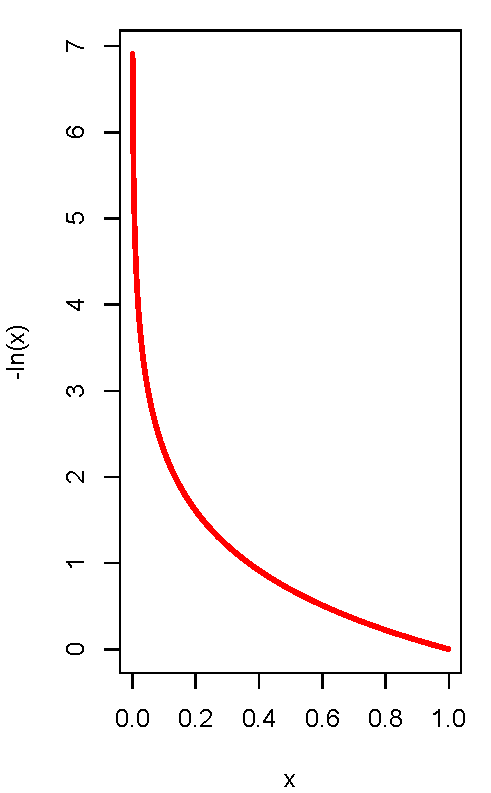
\includegraphics[width=\textwidth]{figures/neg_log}
}
{
\pause
In order to use the previous theorem, need to check the function $g(x) = -\ln(x)$
\begin{enumerate}
\item monotonic \uncover<3->{\checkmark}
\item differentiable \uncover<4->{\checkmark}
\end{enumerate}
\uncover<5->{
Inverse function $g^{-1}(y)$:
\vspace{-0.3cm}
\[ y = -\ln(x) \Longleftrightarrow x = e^{-y} \]
}
\uncover<6->{
\vspace{-0.5cm}
\[
\frac{dx}{dy} = -e^{-y}
\]
}
\uncover<7->{
Range of $Y$: $y \in [0, \infty)$.
\vspace{-0.3cm}
\begin{align*}
f_Y ( y ) & = f_X(x)  \left|\frac{dx}{dy}\right| = 1 \cdot \left| -e^{-y} \right| = e^{-y}
\end{align*}
}
\uncover<8->{Therefor, $Y$ has an exponential distribution,
\vspace{-0.3cm}
\[ Y \sim \text{Exp}(1) \]
}
}

\end{frame}


%%%%%%%%%%%%%%%%%%%%%%%%%%%%%%%%%%%%%
\begin{frame}

\disc{Let $X$ have pdf $f_X(x)$, where $-\infty < x < \infty$. We want to find the pdf for $Y = |X|$.
Can we use the formula $f_Y ( y ) = f_X(x)  \left|\frac{dx}{dy}\right|$?}
\begin{enumerate}[(a)]
\item Yes
\solnMult{No} \uncover<3->{\hfill $g(x) = |x|$ is not monotonic; also not differentiable at $0$.}
\end{enumerate}
\vspace{0.3cm}
\twocol{0.4}{0.6}{
\uncover<3->{
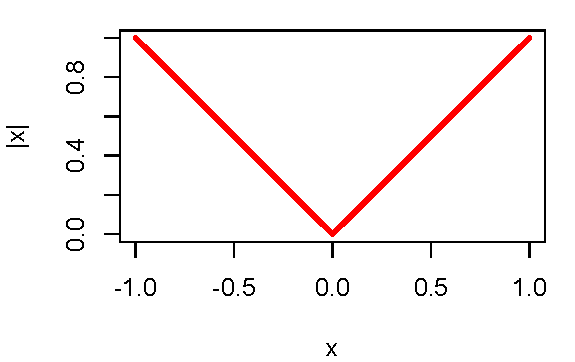
\includegraphics[width=\textwidth]{figures/abs}
}
}
{
\uncover<4->{First find cdf $F_Y(y)$, then find $f_Y(y)$.} \\
\uncover<5->{
For any $y \geq 0$,
\begin{align*}
F_Y(y) & = P(Y < y) \\
&= P(|X| < y) \\
&= P(-y < X < y) \\
& = F_X(y) - F_X(-y)
\end{align*}
}
\uncover<6->{
\vspace{-0.9cm}
\begin{align*}
f_Y(y) & = \frac{d}{dy}[F_X(y) - F_X(-y)]\\
& = f_X(y) + f_X(-y)\\
\end{align*}
}
}

\end{frame}




\end{document}
